\apendice{Especificación de diseño}

\section{Introducción}
En esta sección se describen algunas características relacionadas con el diseño del proyecto.

\section{Diseño de datos}

\subsection{Sensores}
Para este proyecto era necesario la obtención dinámica de datos de sensores en tiempo real, para ello el cliente facilitó una serie de sensores que disponía en una bodega y almacenaba los datos en PRTG, los sensores en cuestión miden el consumo de la bomba de agua \ref{img_Consumo_Bomba_Agua}, la humedad en el ambiente \ref{img_Presion_Tuberia_Agua_PRTG}, la humedad en la parcela \ref{img_Presion_Tuberia_Agua_PRTG} y la presión de la tubería de agua.

\begin{figure}[h]
	\centering
	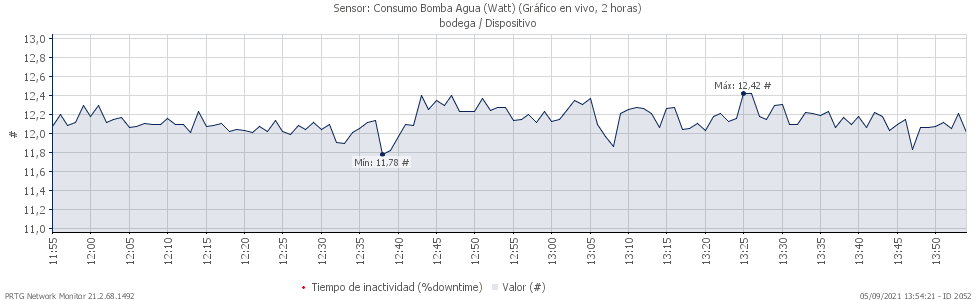
\includegraphics[width=1\textwidth]{img/img_PRTG_Consumo_bomba_agua.png}
	\caption{Sensor del consumo de la bomba de agua}
	\label{img_Consumo_Bomba_Agua}
\end{figure}

\begin{figure}[h]
	\centering
	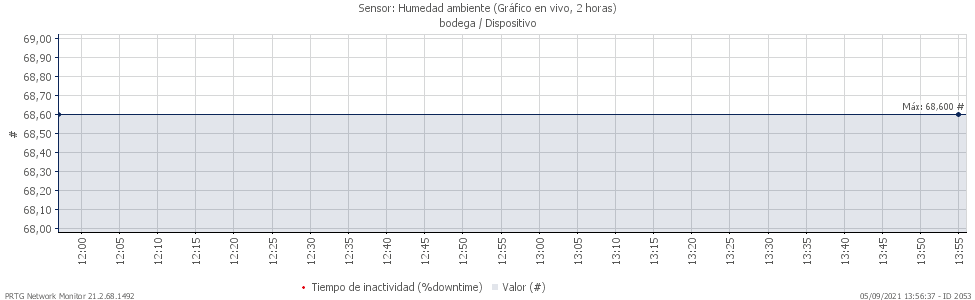
\includegraphics[width=1\textwidth]{img/img_PRTG_Humedad_ambiente.png}
	\caption{Sensor de la humedad en el ambiente}
	\label{mg_Humedad_Ambiente_PRTG}
\end{figure}

\begin{figure}[h]
	\centering
	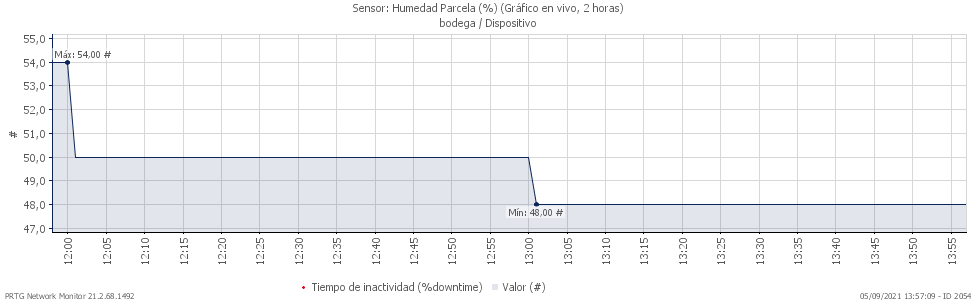
\includegraphics[width=1\textwidth]{img/img_PRTG_Humedad_parcela.png}
	\caption{Sensor de la humedad en la parcela}
	\label{img_Humedad_Parcela_PRTG}
\end{figure}

\begin{figure}[h]
	\centering
	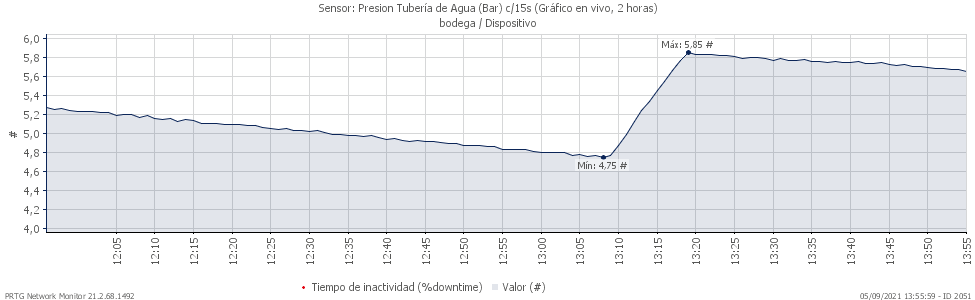
\includegraphics[width=1\textwidth]{img/img_PRTG_Presion_tuberia_agua.png}
	\caption{Sensor de la presión de la tubería de agua}
	\label{img_Presion_Tuberia_Agua_PRTG}
\end{figure}

\newpage
\subsection{Base de datos}

Los datos de los sensores se almacenan en Elasticsearch, una base de datos NoSQL orientada a documentos. A diferencia de las bases de datos relacionales, esta no está estructurada en filas y columnas, Elasticsearch almacena cada registro junto a sus datos asociados en un único documento JSON el cual es asociado a un index Para ver más información sobre la indexación y la estructura de los ficheros consultar el manual de usuario \ref{cap:obt_alm_dato}

\subsection{Diagrama de clases}
 A continuación, se mostrarán los diagramas de clase de la aplicación para facilitar el entendimiento de la estructura del sistema.
 
\begin{figure}[h]
	\centering
	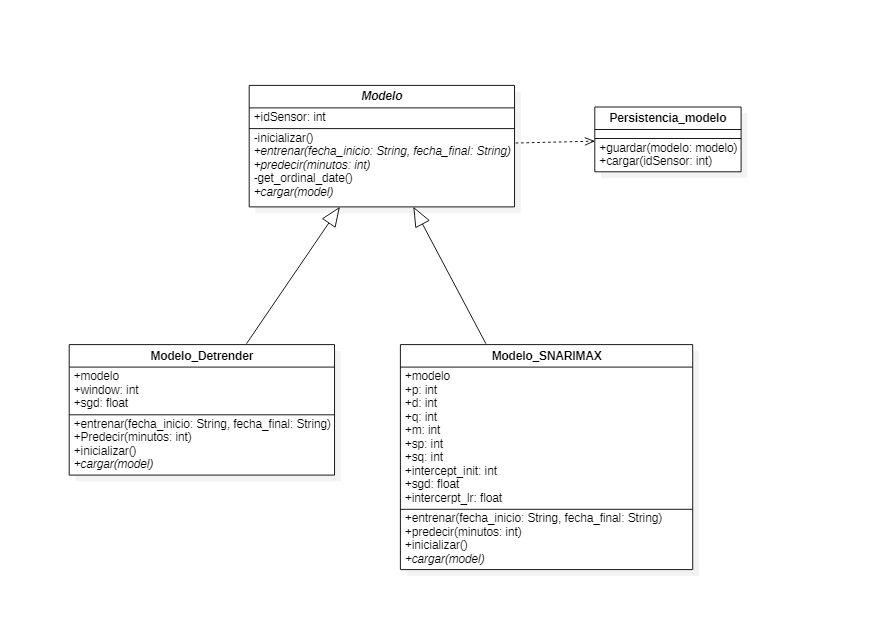
\includegraphics[width=1.1\textwidth]{img/img_diagrama_clases_modelo.png}
	\caption{Diagrama de clases paquete Predicción}
	\label{img_diagrama_clases_modelo}
\end{figure}

\begin{figure}[h]
	\centering
	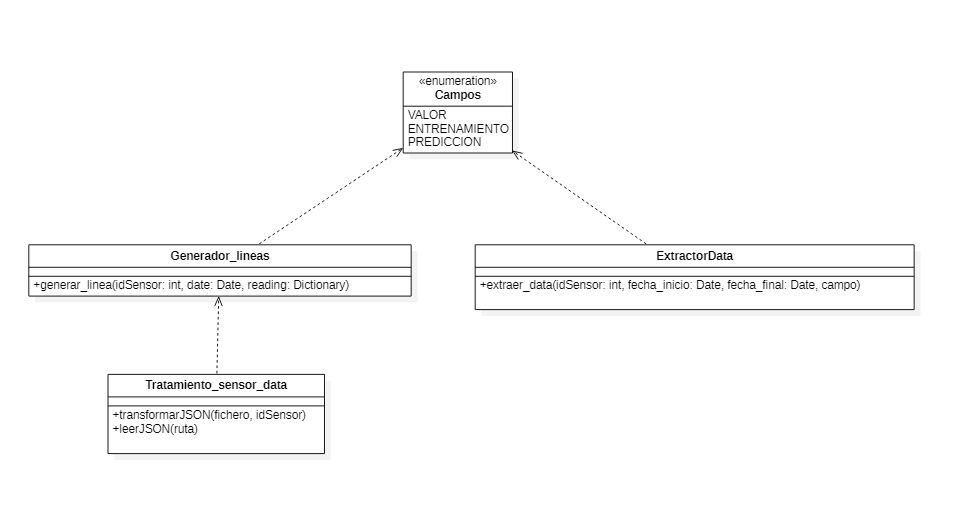
\includegraphics[width=1.1\textwidth]{img/img_diagrama_clases_utilidades.png}
	\caption{Diagrama de clases paquete Utilidades}
	\label{img_diagrama_clases_modelo}
\end{figure}

\newpage

\section{Diseño procedimental}

En este apartado se muestran el diagrama de secuencia

\begin{figure}[h]
	\centering
	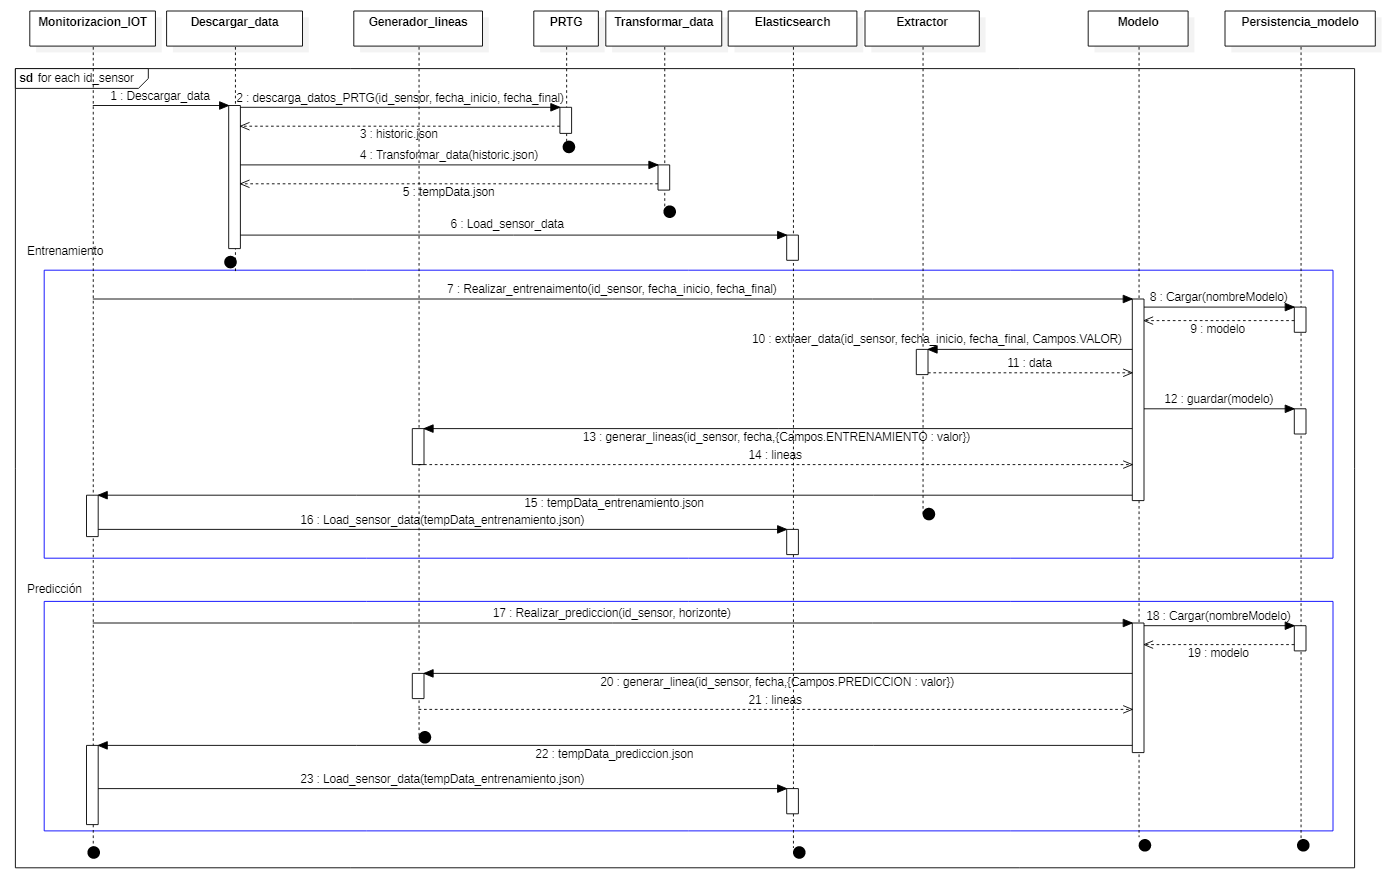
\includegraphics[width=1.1\textwidth]{img/img_diagrama_secuencias.png}
	\caption{Diagrama de secuencias}
	\label{img_diagrama_secuencias}
\end{figure}
\newpage

\section{Diseño arquitectónico}

El proyecto consta de tres paquetes.

\begin{itemize}
    \item \textbf{Gestion\_data}: Este paquete se encarga de todo lo relacionado con la gestión de los datos de los sensores:. 
    \begin{itemize}
        \item Descargar los datos de PRTG.
        \item Subir datos a Elasticsearch.
        \item Descargar datos de Elasticsearch.
        \item Eliminar datos de Elasticsearch.
    \end{itemize}
    
    \item \textbf{Utilidades}: Este paquete se encarga de realizar tareas variadas como:.
        \begin{itemize}
            \item Transformar los ficheros JSON.
        \end{itemize}
    \item \textbf{Prediccion}: Este paquete se encarga de todo lo relacionado con el entrenamiento y la predicción de los sensores:
        \begin{itemize}
            \item Entrenar el modelo.
            \item Realizar la predicción.
            \item Crear modelos.
        \end{itemize}
\end{itemize}

\begin{figure}[h]
	\centering
	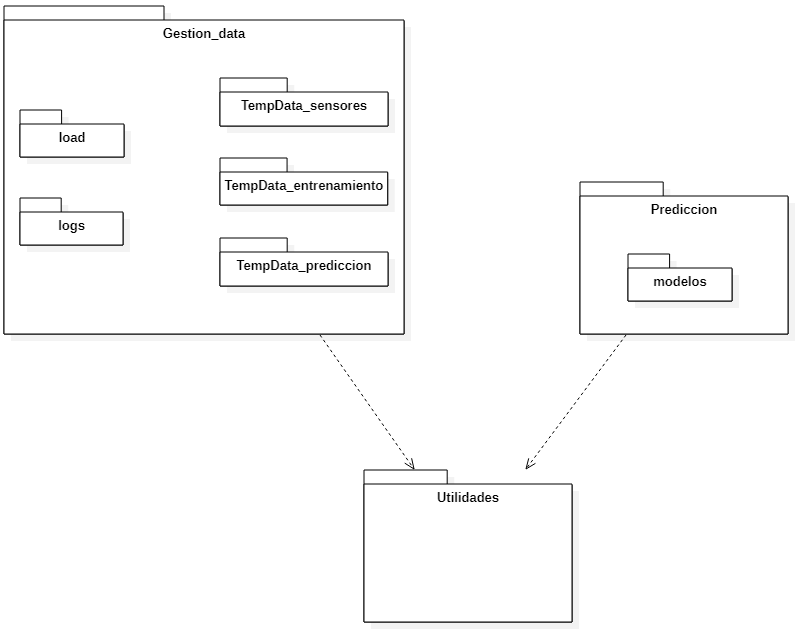
\includegraphics[width=1.1\textwidth]{img/img_diagrama_paquetes.png}
	\caption{Diagrama de paquetes}
	\label{img_diagrama_paquetes}
\end{figure}